\documentclass{article}
\usepackage[catalan]{babel}
\usepackage[latin1]{inputenc}   % Permet usar tots els accents i car�ters llatins de forma directa.
\usepackage{enumerate}
\usepackage{amsfonts, amscd, amsmath, amssymb}
\usepackage{fancyheadings}
\usepackage{graphicx}

\setlength{\textwidth}{16cm}
\setlength{\textheight}{24cm}
\setlength{\oddsidemargin}{-0.3cm}
\setlength{\evensidemargin}{0.25cm} \addtolength{\headheight}{\baselineskip}
\addtolength{\topmargin}{-3cm}

\newcommand\Z{\mathbb{Z}}
\newcommand\R{\mathbb{R}}
\newcommand\N{\mathbb{N}}
\newcommand\Q{\mathbb{Q}}
\newcommand\K{\Bbbk}
\newcommand\C{\mathbb{C}}

\newcounter{exctr}
\setcounter{exctr}{25}
\newenvironment{exemple}
{ \stepcounter{exctr} 
\hspace{0.2cm} 
\textit{Exemple  \arabic{exctr}: }
\it
\begin{quotation}
}{\end{quotation}}

\pagestyle{fancy}
\markboth{Tema 1. Variables aleat\`ories vectorials}{}
\setcounter{page}{12}
\setlength{\headrulewidth}{0pt}

\begin{document}

\noindent
\textbf{\large Variable aleat\`oria Gaussiana bidimensional}

\vskip 0.2 cm
\noindent
Recordatori:
\vskip 0.1 cm
Una v.a. $X$ es diu \textbf{Gaussiana} o \textbf{normal} amb par\`ametres $\mu$ i $\sigma^2$
(i es denota $X \sim \mathrm{N}(\mu, \sigma^2)$), si la seva funci\'o de densitat \'es:
\[
f_X(x)=\frac{1}{\sqrt{2\pi}\sigma}e^{-\frac{(x-\mu)^2}{2 \sigma^2}} , 
\qquad \forall x \in \R
\]

\noindent
La gr\`afica d'aquesta funci\'o s'anomena {\bf campana de Gauss} (veure Figura \ref{campanaGauss}).

\vskip 0.2 cm
\noindent
Propietats:
\begin{itemize}
\item La funci\'o de densitat de la v.a. Gaussiana \'es sim\`etrica respecte a $x=\mu$ i la seva
amplada \'es proporcional a $\sigma$. La gr\`afica d'aquesta funci\'o s'anomena 
{\bf campana de Gauss} (veure Figura \ref{campanaGauss}-esquerra).

\item Si $X \sim N(\mu, \sigma^2)$ llavors $E(X)=\mu$ i $\mathrm{Var}(X)=\sigma^2$.

\item $\mathrm{N}(0, 1)$ rep el nom de {\bf normal est\`andard} i es denota per $\mathrm{Z}$.

\item Les funcions de distribuci\'o d'una normal $X \sim N(\mu, \sigma^2)$ i
la normal es\`andar $Z \sim N(0, 1)$ estan relacionades per la seg\"uent f\`ormula:
\[
F_X(x)=F_Z(\frac{x-\mu}{\sigma})
\]
Com que els valors de $F_Z$ estan tabulats, gr\`acies a aquesta relaci\'o 
es pot con\`eixer el valor de $F_X$ per a una v.a. normal amb par\`ametres qualssevol.

\item En problemes d'Enginyeria els valors de probabilitat de la v.a. Gaussiana es 
solen calcular utilitzant les funcions $\mathrm{erf}(x)$ i $\mathrm{erfc}(x)$, 
les quals es troben tabulades:
\[
F_X(x)=P(X \leq x)=\frac{1}{2} \mathrm{erf}(\frac{x-\mu}{\sqrt{2} \sigma})=
\frac{1}{2} \mathrm{erfc}(\frac{\mu-x}{\sqrt{2} \sigma})
\]


\end{itemize}

\begin{figure}[htbp]
\begin{center}
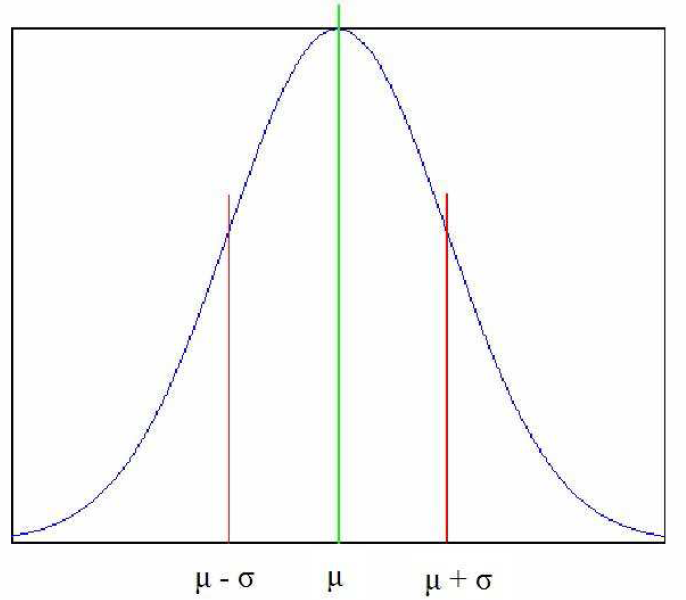
\includegraphics[width=5cm]{normalpdf.png} 
$\qquad \qquad$
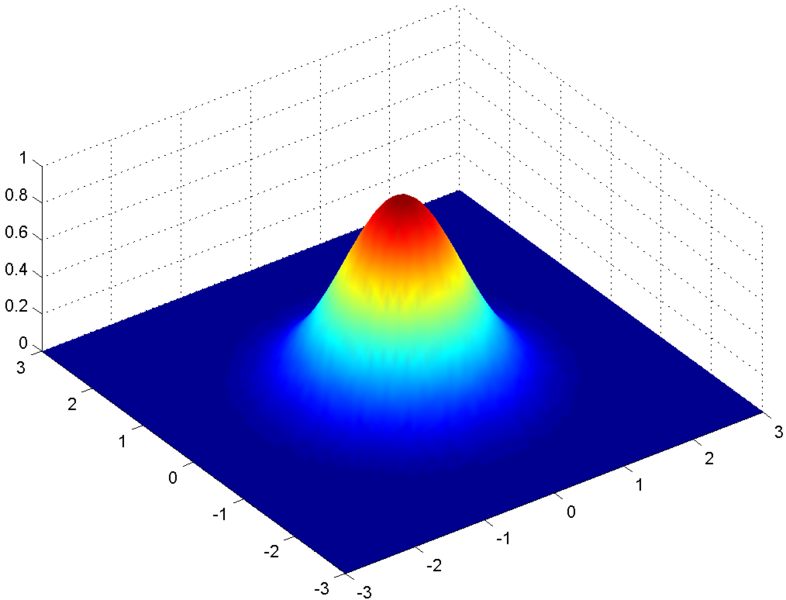
\includegraphics[width=7cm]{786px-Gaussian_2d.png}
\caption{Esquerra: campana de Gauss. Dreta: campana de Gauss bidimensional (font: wikipedia).}
\label{campanaGauss}
\end{center}
\end{figure}



\newpage
\noindent
En aquest tema:
\vskip 0.1 cm
dues variables aleat\`ories $X$ i $Y$ es diu que s\'on \textbf{conjuntament Gaussianes} si la seva funci\'o de
densitat conjunta \'es:
\[
f_{XY}(x, y)=\frac{1}{2 \pi \sigma_X \sigma_Y \sqrt{1-\rho_{XY}^2}} \,
e^{- \frac{1}{2(1-\rho_{XY}^2)} \left[ (\frac{x-\mu_X}{\sigma_X})^2 + (\frac{y-\mu_Y}{\sigma_Y})^2 - 
2 \rho_{XY} (\frac{x-\mu_X}{\sigma_X}) (\frac{y-\mu_Y}{\sigma_Y}) \right]}
\]
\noindent
La gr\`afica d'aquesta funci\'o es mostra en la figura \ref{campanaGauss}-dreta.


\vskip 0.3 cm
Propietats:
\begin{itemize}
\item Si $(X, Y)$ s\'on conjuntament Gaussianes amb l'anterior funci\'o de densitat conjunta, 
llavors: $E(X)=\mu_X$, $E(Y)=\mu_Y$, $\mathrm{Var}(X)=\sigma_X^2$, $\mathrm{Var}(Y)=\sigma_Y^2$ i el
coeficient de correlaci\'o de les variables \'es $\rho_{XY}$.

\item Una manera m\'es compacta d'escriure l'anterior funci\'o de densitat \'es, amb notaci\'o matricial:
\[
f_{XY}(x, y)=\frac{1}{\sqrt{2 \pi \, \mathrm{det}(K)}} \, e^{-\frac{1}{2} 
\begin{pmatrix} x-\mu_X & y - \mu_Y \end{pmatrix} K^-1 \begin{pmatrix} x-\mu_X \\ y - \mu_Y \end{pmatrix}}
\]
\noindent
on $K$ \'es la matriu de covari\`ancies de $X$ i $Y$: 
$K=\begin{pmatrix} \sigma_X^2 & \sigma_{XY} \\ \sigma_{XY} & \sigma_Y^2 \end{pmatrix}$.

\item Si $(X, Y)$ s\'on conjuntament Gaussianes amb l'anterior funci\'o de densitat conjunta, llavors
les funcions de densitat marginals s\'on tamb\'e Gaussianes: 
$X\sim N(\mu_X, \sigma_X^2)$ i $Y \sim N(\mu_Y, \sigma_Y^2)$.

\item Si $(X, Y)$ s\'on conjuntament Gaussianes, llavors les funcions de densitat condicionals 
$f_{Y|X}(y|x)$ i $f_{X|Y}(x|y)$ s\'on tamb\'e Gaussianes.

\item Si $(X, Y)$ s\'on conjuntament Gaussianes i 
$\begin{pmatrix} U \\ V \end{pmatrix}=A \cdot \begin{pmatrix} X \\ Y \end{pmatrix}$, amb $\mathrm{det}(A)\neq 0$,
llavors $(U, V)$ s\'on conjuntament Gaussianes.

\item Si $(X, Y)$ s\'on conjuntament Gaussianes, llavors $Z=a_1 X+ a_2 Y$ \'es una v.a. Gaussiana per a 
qualsevol valor de les constants $a_1$ i $a_2$.

\end{itemize}



\end{document}
